\section{Problem solving}
In this section, we first introduce the uniform random sampling algorithm for visualization-aware sampling problem in Section~\ref{sec:random}.
We then propose a greedy algorithm for it in Section~\ref{sec:greedy}.
However, both random sampling algorithm and greedy algorithm do not guarantee the approximate ratio of the visualization result.
We then propose an approximate algorithm for it in Section~\ref{sec:app}.

\subsection{Uniform Random Sampling}~\label{sec:random}
The straight forward solution for the visualization-aware sampling problem is randomly select $k$ trajectories from $\D$, 
then render these selected $k$ trajectories into the canvas.
The uniform random sampling algorithm has excellent performance.
However, the trade-off is that it does not provide any guarantee on the visualization results.
Trajectory data $\D$\cite{xxx} consists of almost 10K trajectories which collected by Didi company.
The visualization result of the whole dataset $\D$ is illustrated in Figure~\ref{fig:demo}(b).
Figure~\ref{fig:demo}(b) shows the visualization result of uniform random sampling result of $\D$ with $k=100$.
The difference between the visualization results in Figures~\ref{fig:demo}(a) and (b) are obvious from user's perspective.

\begin{figure}
 \centering
 \small
 \begin{tabular}{cc}
   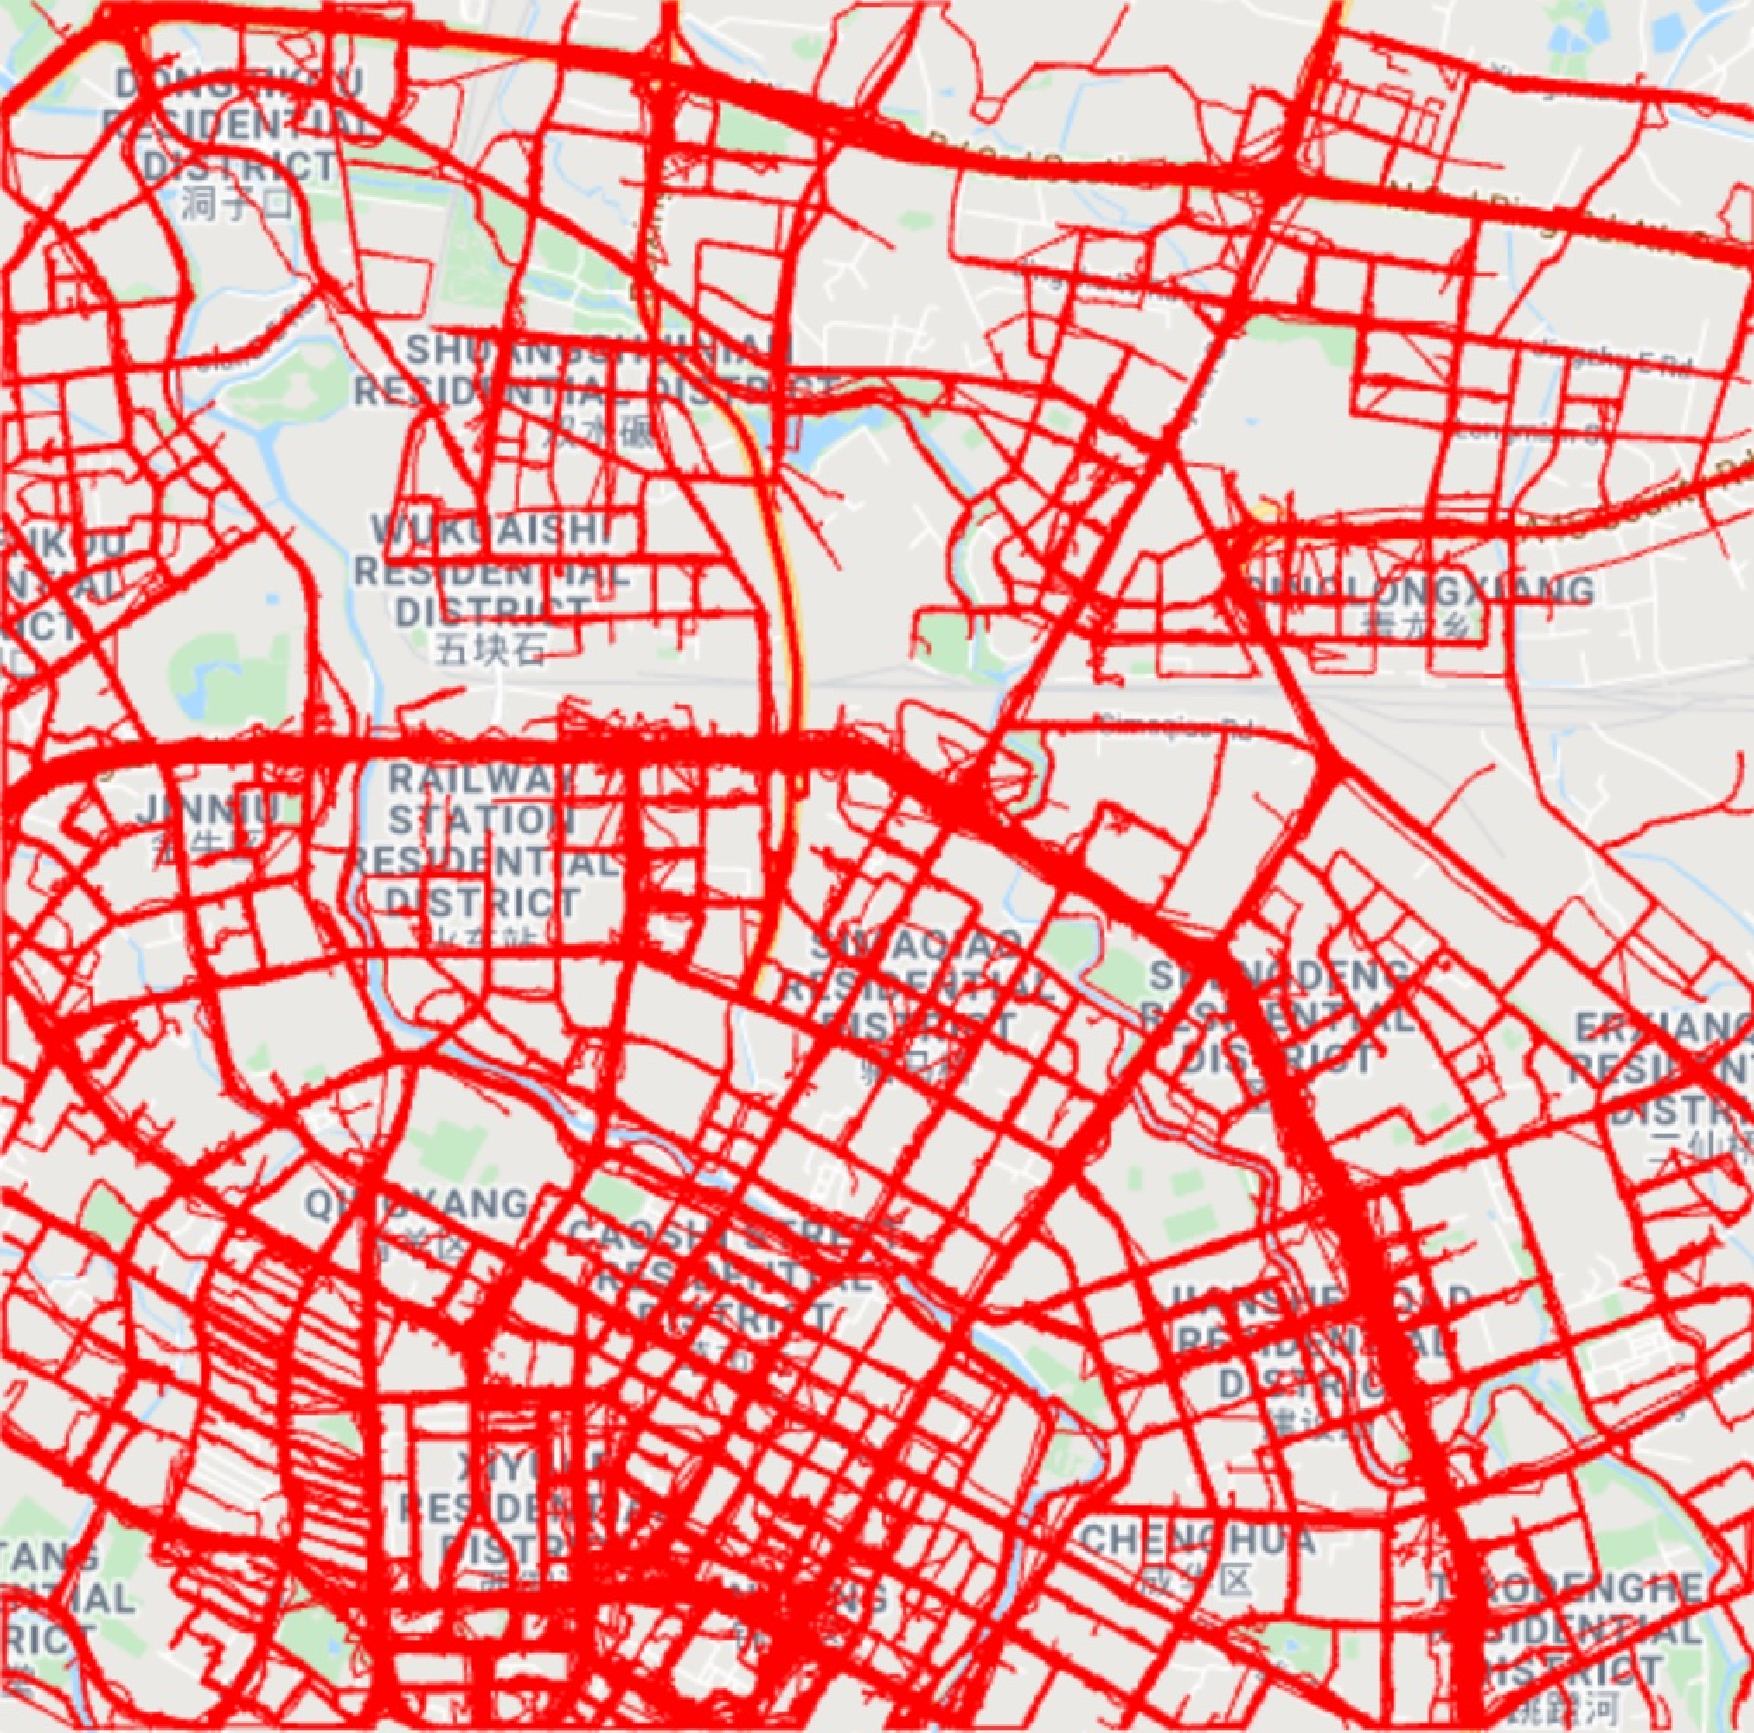
\includegraphics[width=0.45\columnwidth]{chengdu_total}
   &
   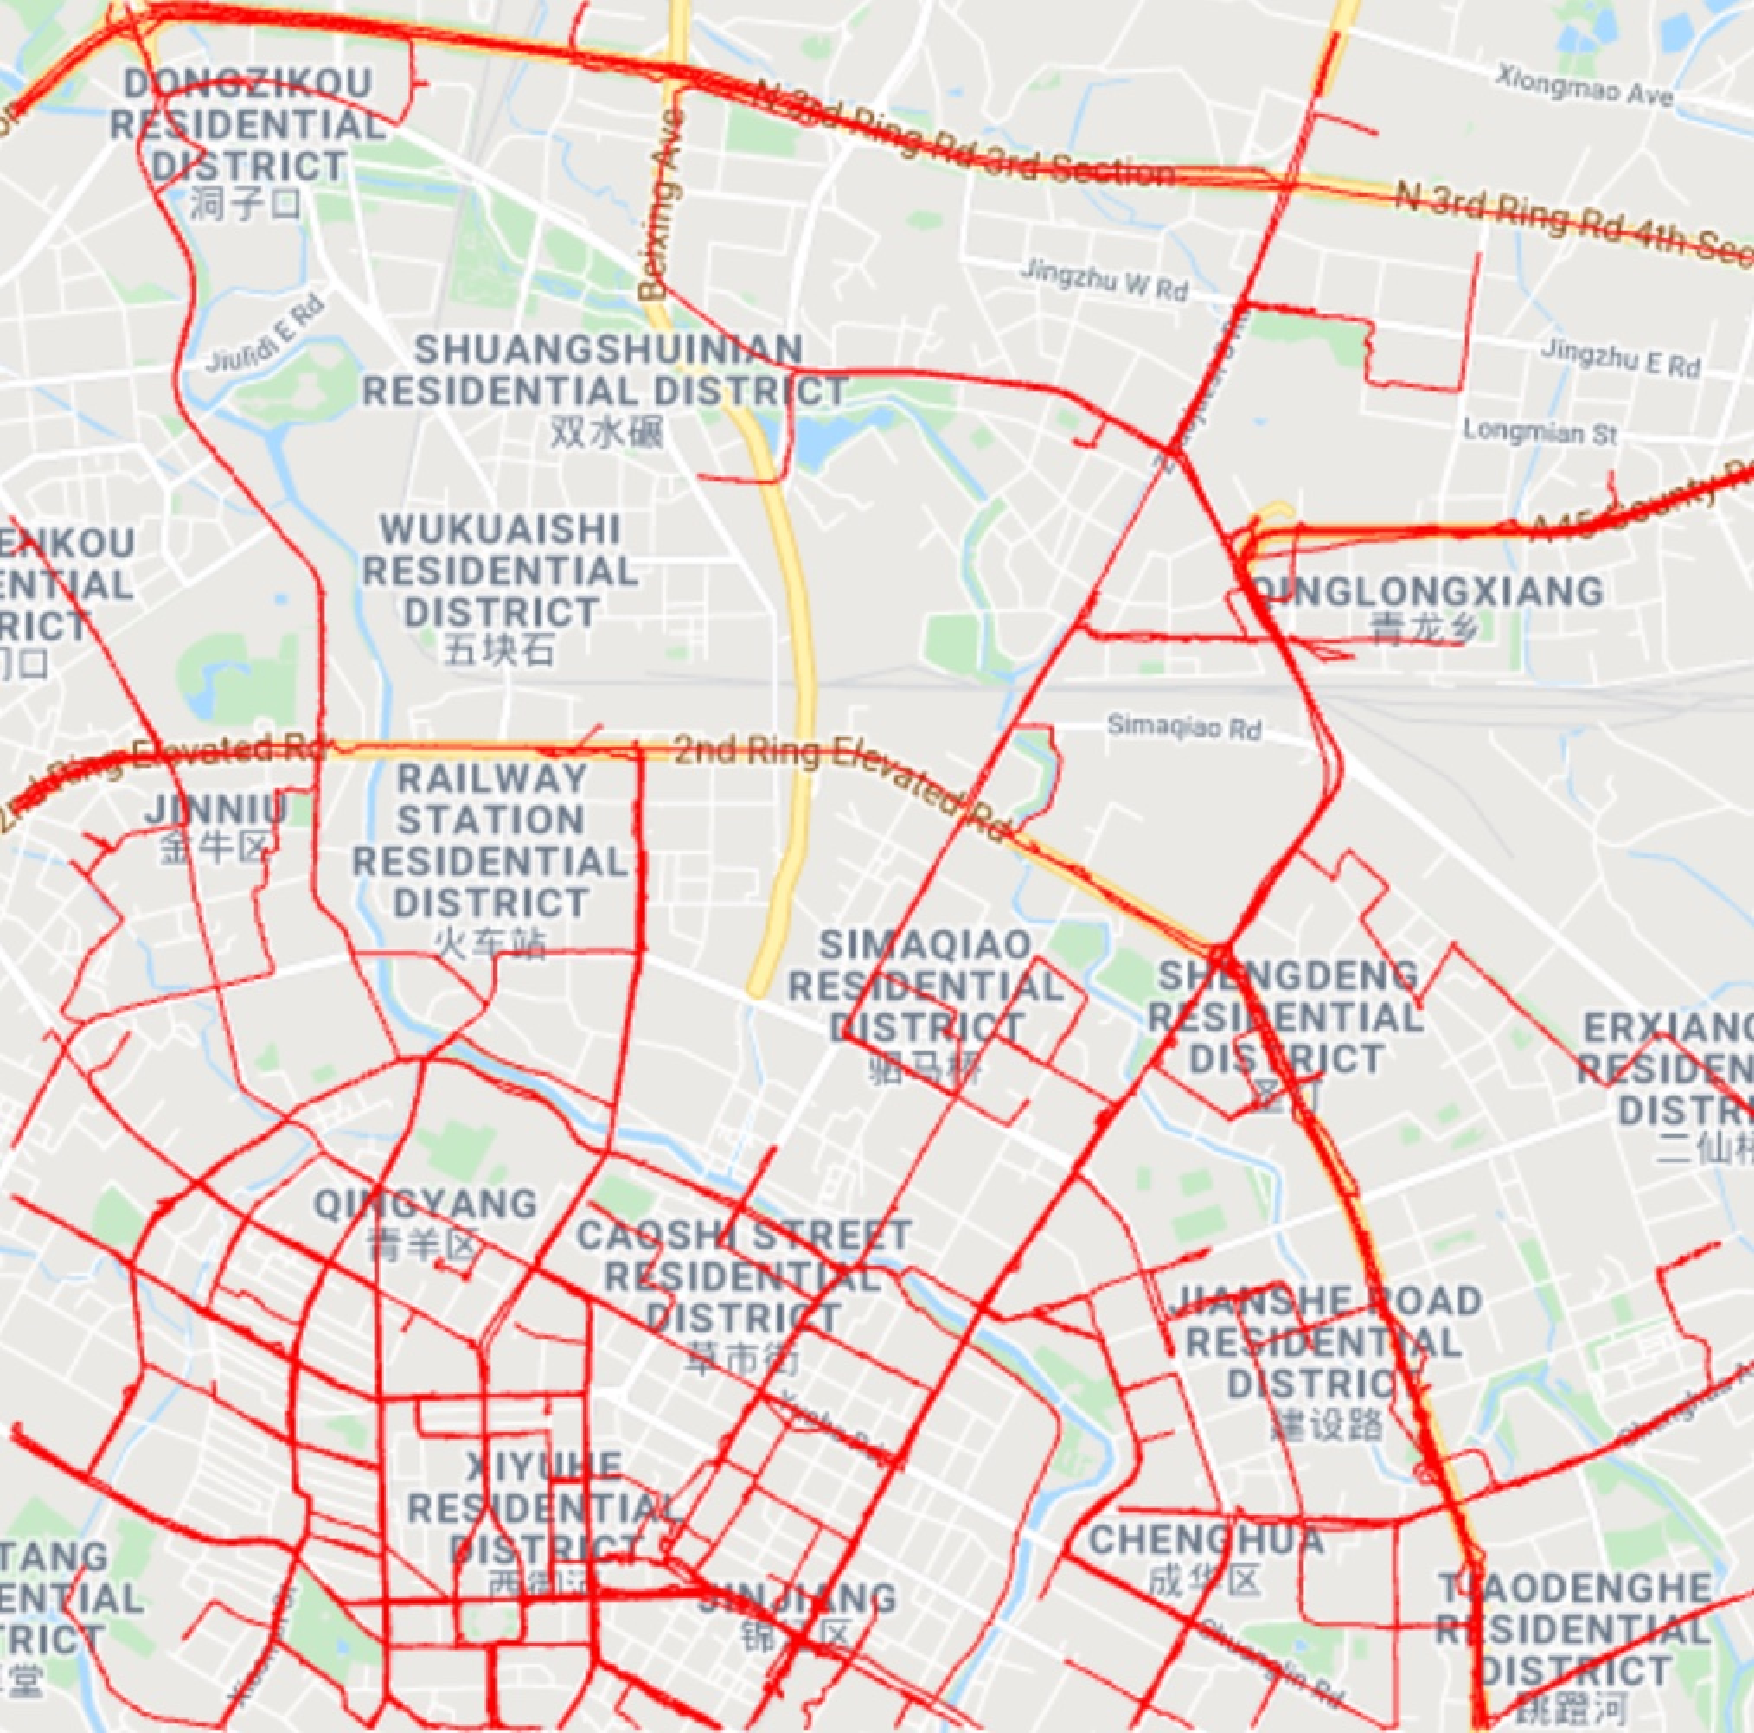
\includegraphics[width=0.45\columnwidth]{chengdu_sampling}
   \\
   (a) Dataset $\D$
   &
   (b) Uniform sampling $\oR$
 \end{tabular}
 \caption{Visualization results of trajectory set in Chengdu}
 \label{fig:demo}
\end{figure}

\subsection{Greedy Algorithm}~\label{sec:greedy}
In order to improve the visualization quality of visualization-aware sampling problem, we devise greedy algorithm in this section.
In general, the visualization result quality is related to the user zoom level.
For example, Google map\footnote{\url{https://www.google.com/maps/preview}} provides levels range from 0 to 20, 
where level 0 is the lowest level (e.g., the whole world), level 20 is the highest level (e.g., individual building, if available).
The size of each pixel in the canvas is defined by the highest zoom level.
For each trajectory $\D_i in \D$ is a set of pixels in the canvas.
The pesudocode of the greedy algorithm is presented in Algorithm~\ref{alg:greedy}.
Specifically, it finds the trajectory $\D_i$ in $\D$ which maximize the union set of $\oR \cup \D_i$ at each iteration.
It terminates after $k$ iterations and returns $\oR$ to graphics device for rendering.

\begin{algorithm}
    \caption{Greedy($\D$,k)} \label{alg:greedy}
    \begin{algorithmic}[1]
    \State Initialize result set $\oR \leftarrow \emptyset$
    \While{$|\oR| < k$}
        \State $\oR_{tmp} \leftarrow argmax_{\D_i \in \D} \oR \cup \D_i$
        \State $\oR \leftarrow \oR \cup \{ \oR_{tmp} \}$
    \EndWhile
    \State Return $\oR$
    \end{algorithmic}
\end{algorithm}

\begin{theorem}~\label{the:ratio}
Algorithm~\ref{alg:greedy} provides a $1-(1-1/k)^k \geq (1-1/e) \approx 0.632$ approximation result for the visualization-aware sampling problem.
\end{theorem}

\subsection{Performance Optimizations}


\Bo{Direction I (for visual performance): pixel cover criteria, i.e., if we render pixels at $(x,y)$, then all pixels in $[(x-\delta, y-\delta), (x+\delta, y+\delta)]$ will be skipped directly.}

\Bo{Direction II (for time cost): trajectory representation, i.e., we formulate the universal set by the roads in the map, then, before we call road-matching to generate the set of each trajectory,
after that we then incurs greedy algorithm.}
